
\textbf{Introduction}\\

Tout au long de ce chapitre, nous allons traiter
les histoires utilisateurs de notre premier sprint "Gestion de thème de formation" pour produire un ensemble d’incréments potentiellement
livrable. Avant de se lancer dans le premier sprint, il s'agit de définir le but de ce dernier qui doit
être défini en terme métier et non pas en terme technique pour qu’il soit compréhensible par les membres
en dehors de l’équipe. Il s’agit de répondre à une question fondamentale «pourquoi faisons-nous
ce sprint ?».

\section{Sprint Planning Meeting}
\subsection{Objectif de sprint}
Au cours de ce premier sprint, nous allons développer les fonctionnalités reliées au EPIC:

	 Gestion de thème de formation

Le développement du sprint doit obligatoirement passer par les étapes suivantes: Analyse, conception et réalisation.

\subsection{Backlog du premier sprint}
Elaboration du sprint backlog du sprint 1 à partir du Backlog product comme présentée dans le
tableau suivant.
\newpage
\begin{table}[!h]
	\centering % used for centering table
	\begin{tabular}{|c|p{5cm}|p{8cm}|c|}
		\hline
		\textbf{Id}&\textbf{User Story} & \centering{\textbf{Sprint Backlog Item}} & \textbf{Effort}\tabularnewline
		\hline
	 \multirow{2}{*}{US1}&\multirow{2}{4cm}{En tant qu'administrateur, je peux créer un thème }&Créer un nouveau type de contenu personnalisé nommé "Events"&3\\
	 \cline{3-4}
	 &&Développer un "must use plugin" &5\\
	 \hline
	  \multirow{2}{*}{US2}&\multirow{2}{4cm}{En tant qu'utilisateur, je peux consulter la liste des thèmes (All Events) }&Ecrire une requête personnalisée pour afficher le nouveau type de contenu créé sur l'interface du site web&3\\
	 \cline{3-4}
	 &&Réaliser l'interface de la page "All Events" &5\\
	 \hline
	  \multirow{4}{*}{US3}&\multirow{4}{4cm}{En tant qu'administrateur, je peux mettre à jour un thème }&Installer et activer le plugin Advanced Custom Fields (ACF)&3\\
	 \cline{3-4}
	  &&Créer un group de champs "Event Date" &3\\
	 \cline{3-4}
	 &&Développer la fonction qui permet de mettre à jour un thème &3\\
	 \cline{3-4}
	
	  &&"Tester" &2\\
	 \hline
	 \multirow{2}{*}{US4}&\multirow{2}{5cm}{En tant qu'utilisateur, je peux consulter les détails d'un thème} & Réaliser l'interface de la page détails thème &3\\
	 \cline{3-4}
	 &&Développer la fonction qui permet de lister et consulter tous les évènements passés &5\\
	 \hline
	 
	  
		
	\end{tabular}
	\caption{Tableau : Backlog Sprint 1}
\end{table}
\textbf{Remarque}\\
"Les estimations de l’effort des différents Sprint Backlog Item représentent une analyse
comparative pour estimer grossièrement les éléments du backlog de produit avec un
dimensionnement relatif.
Dans cette technique d'estimation, chaque estimateur a un ensemble de cartes de poker de
planification de valeurs: 0,1,2,3,5,8,13,20,40 et 100.
Après les discussions, tous les estimateurs sont invités à sélectionner une carte pour estimer
une user story. Si tous les estimateurs donnent la même valeur, alors cela devient
l'estimation finale.
Si les valeurs sont différentes, les estimateurs donnant les valeurs les plus élevées et les plus
basses expliquent leurs opinions et pourquoi ils ont choisi cette valeur, jusqu'à ce qu'un
consensus soit atteint."\footnote{I.AMMARI, cours Projet d’intégration, ISET Rades 2021-2022 }
\section{Analyse}
\subsection{Diagramme de cas d'utilisation}
Il s'agit de la première étape du sprint 1. Avant de créer une formation l'administrateur doit fixer tout d'abord le thème de formation.  
La figure suivante illustre le diagramme de cas d’utilisation « Gestion thème » du premier Sprint.
\newpage
\begin{itemize}
\item Diagramme de cas d'utilisation global du sprint 1:
\begin{figure}[!h]
	\centering
	{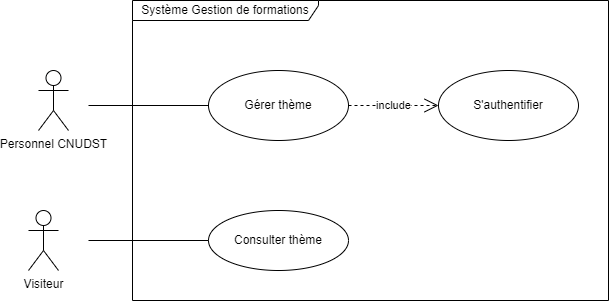
\includegraphics[width=0.85\textwidth]{D) IMAGES/globtheme.png}}
	\caption{Diagramme cas d'utilisation globale -sprint 1}
	\label{Org}
\end{figure}
\item Détails du cas d'utilisation globale Gérer thème
\begin{figure}[!h]
	\centering
	{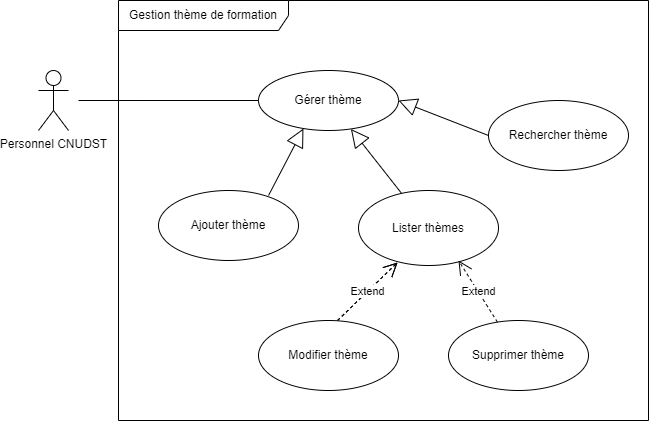
\includegraphics[width=0.85\textwidth]{D) IMAGES/CasUtilisationsprint1.png}}
	\caption{Détails du cas d'utilisation globale Gérer thème}
	\label{Org}
\end{figure}
\newpage
\item Détails de cas d'utilisation globale Consulter thème de formation 

\begin{figure}[!h]
	\centering
	{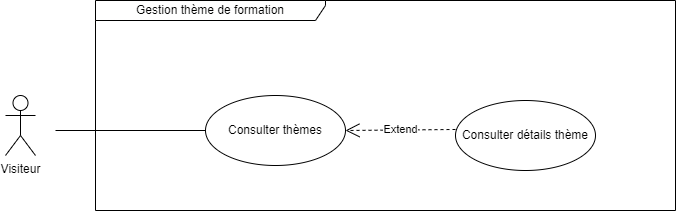
\includegraphics[width=0.85\textwidth]{D) IMAGES/constheme.png}}
	\caption{Détails de cas d'utilisation globale Consulter thème de formation}
	\label{Org}
\end{figure}
\end{itemize}
\section{Description textuelle des cas d'utilisation}
\subsection{Description textuelle des cas d’utilisation:Ajouter thème}
\textbf{Acteur Principal:} L'administrateur\\
\textbf{Date de Création:}08/05/2022\\
\textbf{Date de mise à jour:}10/05/2022\\
\textbf{Responsable:} CNUDST\\
\textbf{Version:}1\\
\textbf{Description des Scénarii:}\\
Le cas d'utilisation commence quand un administrateur décide de créer un thème de formation\\
\textbf{Précondition:} L'administrateur décide de créer un thème de formation.\\
\textbf{Scénario nominal:}
\begin{enumerate}
	\item L'administrateur entre le titre du thème.
	\item L'administrateur entre la description du thème.
	\item L'administrateur clique sur le bouton "ajouter".
	\item Le système vérifie les données saisies.
	\item Le thème est ajouté au niveau de la base des données.
	
\end{enumerate}
\textbf{Scénario Alternatif A:} A1: Un des champs (titre ou description) non rempli, l'enchaînement A1 démarre au point 4 du scénario nominal.\\
Le système affiche le formulaire en indiquant qu'il y a un ou deux champs non remplis.

\subsection{Description textuelle des cas d’utilisation:Lister et mettre à jour un thème}
\textbf{But}: Détailler les étapes permettant à l'administrateur d'afficher la liste des thèmes et d'y effectuer des opérations de gestion (modification et suppression).\\
\textbf{Acteur Principal:} Administrateur \\
\textbf{Date de Création:}28/05/2022\\
\textbf{Date de mise à jour:}31/05/2022\\
\textbf{Responsable:} Olfa CHAOUECH\\
\textbf{Version:}1.0\\
\textbf{Description des Scénarii:}\\
Le cas d'utilisation commence quand l'administrateur est connecté et veut lister les thèmes ou bien mettre à jour un thème.\\
\textbf{Précondition:} L'administrateur décide de consulter un thème de formation.\\
\textbf{Scénario nominal:}
\begin{enumerate}
	\item L'administrateur clique sur le type de contenu Events afin de gérer les thèmes.
	\item Le système récupère les données des thèmes de la base.
	\item Le système affiche la liste de tous les thèmes disponibles et en face de chacun il existe deux options: un bouton "Edit" et un bouton "Delete".
	\item L'administrateur consulte la liste des thèmes.
	\item L'administrateur choisit un thème et une option:\\
	\textbf{Modification:}
	\begin{enumerate}
		\item L'administrateur clique sur "Edit".
		\item Le système affiche une interface de mise à jour.
		\item L'administrateur clique sur "update".
	\end{enumerate}
	\textbf{Suppression}
	\begin{enumerate}
		\item L'administrateur clique sur le bouton "Supprimer".
		\item Le système supprime le thème de la base.
	\end{enumerate}
	
\end{enumerate}
\textbf{Scénario Alternatif A:} \\
A1: L'administrateur est sur la page de mise à jour de thème et veut modifier un autre.\\ 	$\rightarrow$l'enchaînement A1 démarre au point 5-a du scénario nominal.\\
\textbf{Scénario d'exception E:}\\
E1 :L'administrateur change d'avis et veut abandonner la consultation des thèmes et les opérations de mise à jour.\\
	$\rightarrow$L'enchaînement E1 démarre au point 4 du scénario nominal.\\
5- L'administrateur termine sa visite en quittant la page.

\subsection{Description textuelle des cas d’utilisation:Consulter thème}
\textbf{But}: Détailler les étapes permettant à un visiteur d'afficher la liste des thèmes et de consulter chaque thème.\\
\textbf{Acteur Principal:} Visiteur \\
\textbf{Date de Création:}17/05/2022\\
\textbf{Date de mise à jour:}19/05/2022\\
\textbf{Responsable:} Olfa CHAOUECH\\
\textbf{Version:}1.0\\
\textbf{Description des Scénarii:}\\
Le cas d'utilisation commence quand un utilisateur visite notre site.\\
\textbf{Précondition:} Le visiteur décide de consulter un thème de formation.\\
\textbf{Scénario nominal:}
\begin{enumerate}
	\item Le visiteur consulte la rubrique "View All Events" ou "Events".
	\item Le système affiche la liste de tous les thèmes disponibles.
	\item le visiteur choisit un thème et clique dessus.
	\item Le système redirige le visiteur vers la page du thème choisi.
	\item Le système affiche les détails de ce thème.
	
\end{enumerate}
\textbf{Scénario Alternatif A:} \\
A1: Le visiteur est sur la page d'un thème et veut consulter les autres thèmes disponibles,\\ 	$\rightarrow$l'enchaînement A1 démarre au point 2 du scénario nominal.\\
\textbf{Scénario d'exception E:}\\
E1 : Le visiteur ne trouve pas le thème souhaité sur la liste.\\
	$\rightarrow$L'enchaînement E1 démarre au point 2 du scénario nominal.\\
3- Le visiteur quitte la page.

\section{Conception}
\subsection{Diagramme de classes}
Afin d'exprimer la structure statique de modélisation des données d'un système, nous allons utiliser le diagramme de classes. Ce dernier représente une description qui permet de montrer sa structure interne sous forme des classes et des relations entre elles.

\begin{figure}[!h]
	\centering
	{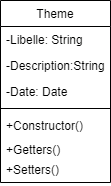
\includegraphics[width=0.15\textwidth]{D) IMAGES/classe1.png}}
	\caption{diagramme de classe -sprint 1}
	\label{Org}
\end{figure}
\newpage
\subsection{Diagramme de séquences}
\begin{itemize}
	\item diagramme de séquences de cas d'utilisation "Ajouter thème"
\begin{figure}[!h]
	\centering
	{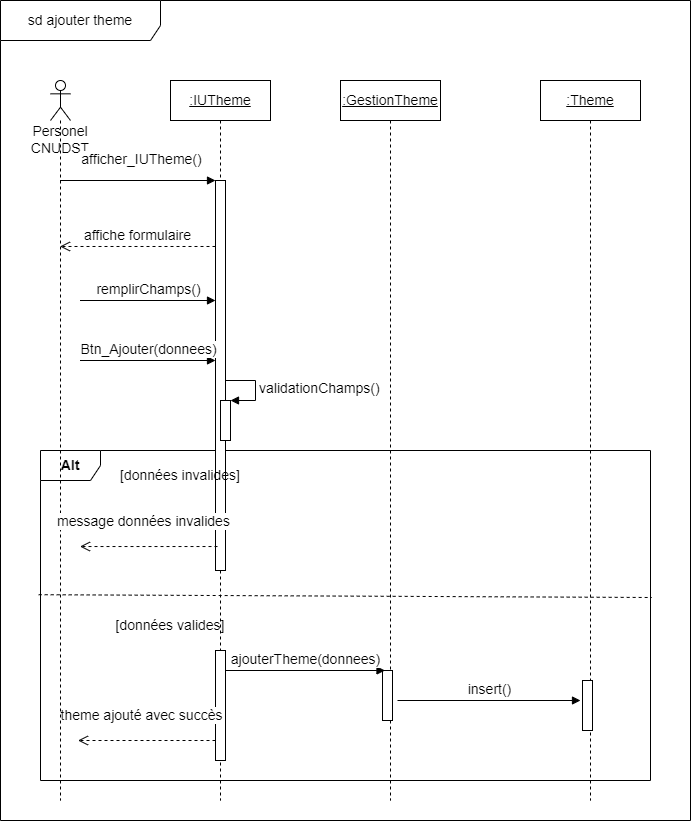
\includegraphics[width=0.75\textwidth]{D) IMAGES/diagseq1.png}}
	\caption{diagramme de séquences de cas d'utilisation "Ajouter thème"}
	\label{Org}
\end{figure}
\item diagramme de séquences de cas d'utilisation "Lister thème"
\begin{figure}[!h]
	\centering
	{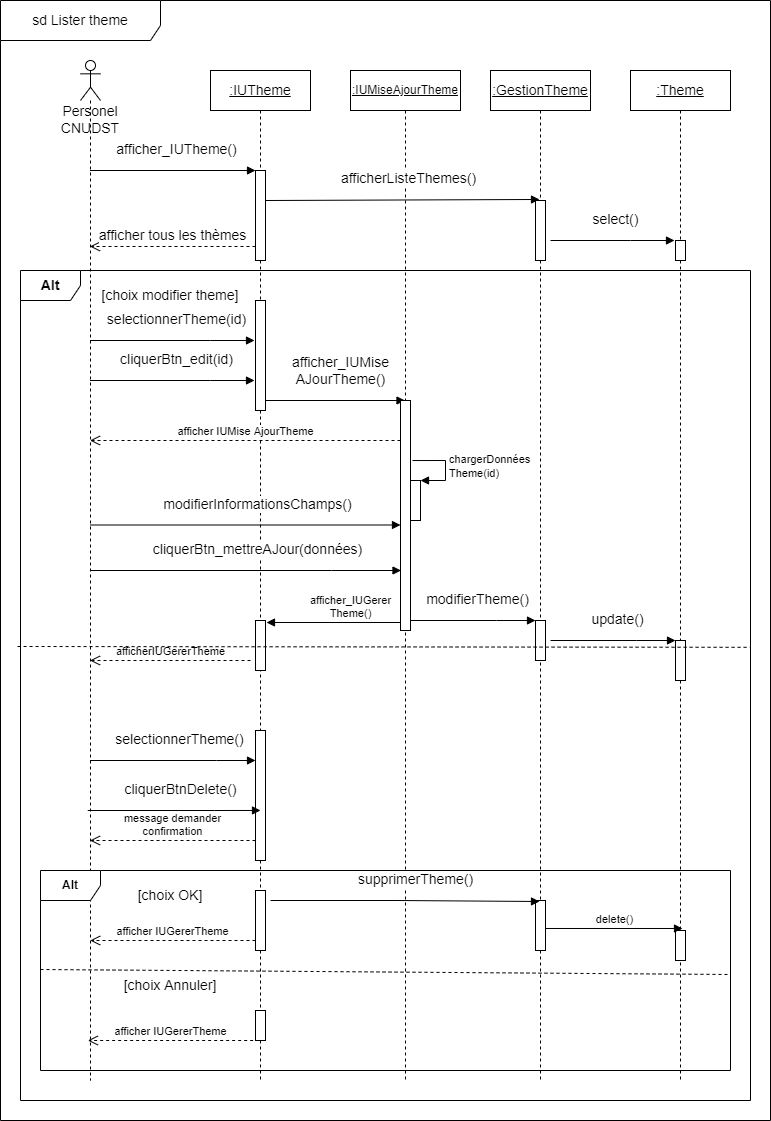
\includegraphics[width=0.75\textwidth]{D) IMAGES/diagSeqLister.png}}
	\caption{diagramme de séquences de cas d'utilisation "Lister thème"}
	\label{Org}
\end{figure}
\newpage
\item diagramme de séquences de cas d'utilisation "Consulter thème"
\begin{figure}[!h]
	\centering
	{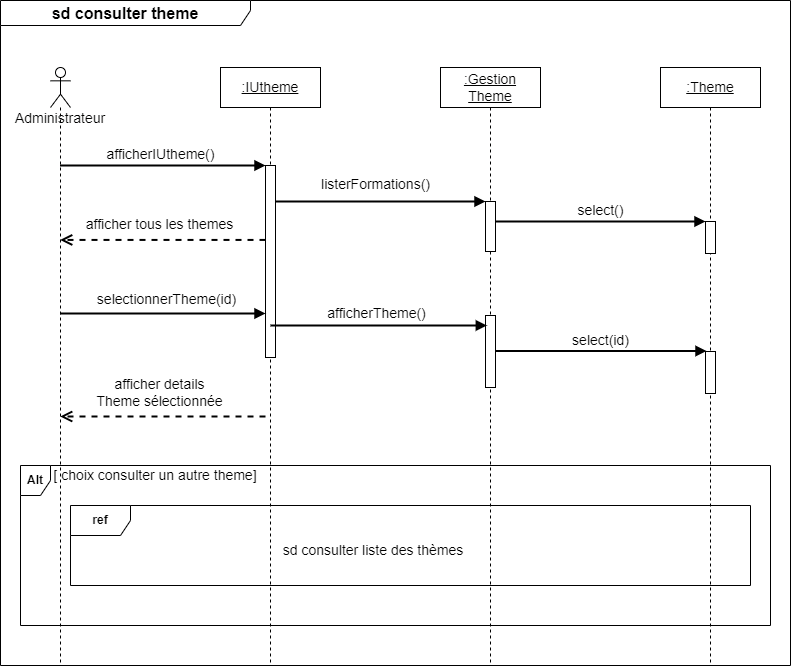
\includegraphics[width=0.75\textwidth]{D) IMAGES/diagconstheme.png}}
	\caption{diagramme de séquences de cas d'utilisation "Consulter thème"}
	\label{Org}
\end{figure}

\newpage
\end{itemize}
\subsection{Réalisation}
Dans cette sous-section, nous présentons la partie réalisation de l’application et la mise en œuvre des
différents composants décrits ci-dessus.
\begin{figure}[!h]
	\centering
	{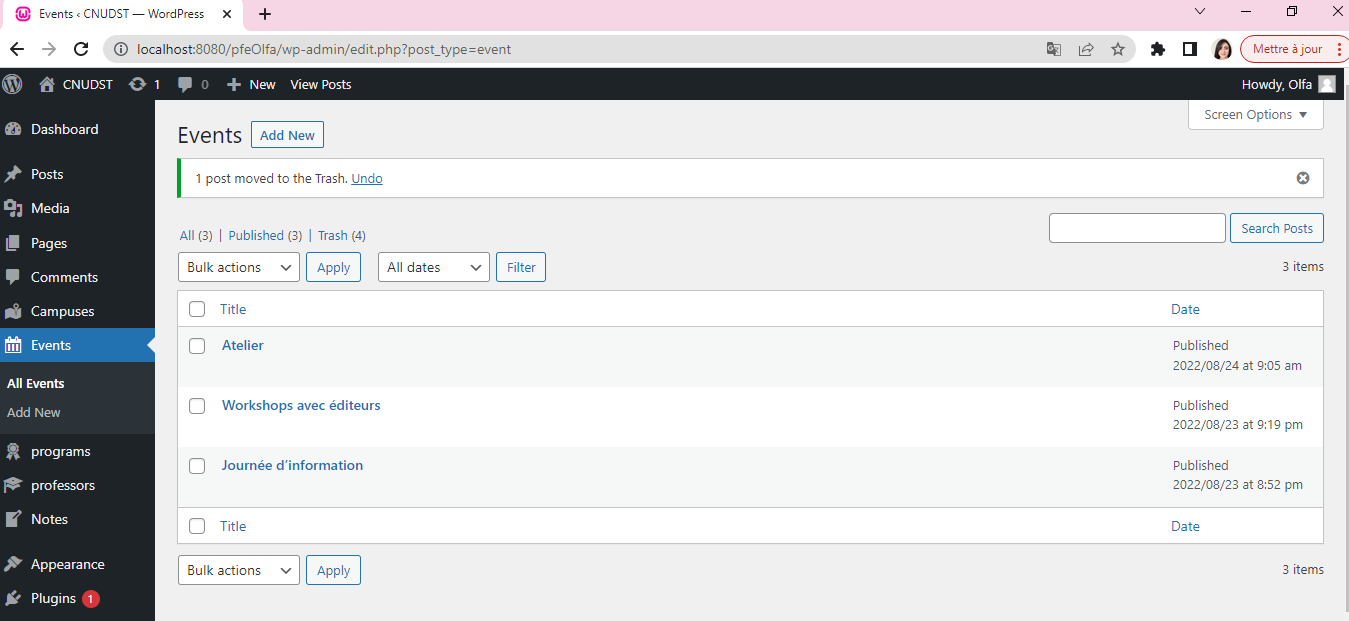
\includegraphics[width=1\textwidth]{D) IMAGES/ajouterTheme.png}}
	\caption{Ajouter thème}
	\label{Diagramme3}
\end{figure}\\
Cette interface permet à un administrateur de créer et de mettre à jour un nouveau thème de formations.

\begin{figure}[!h]
	\centering
	{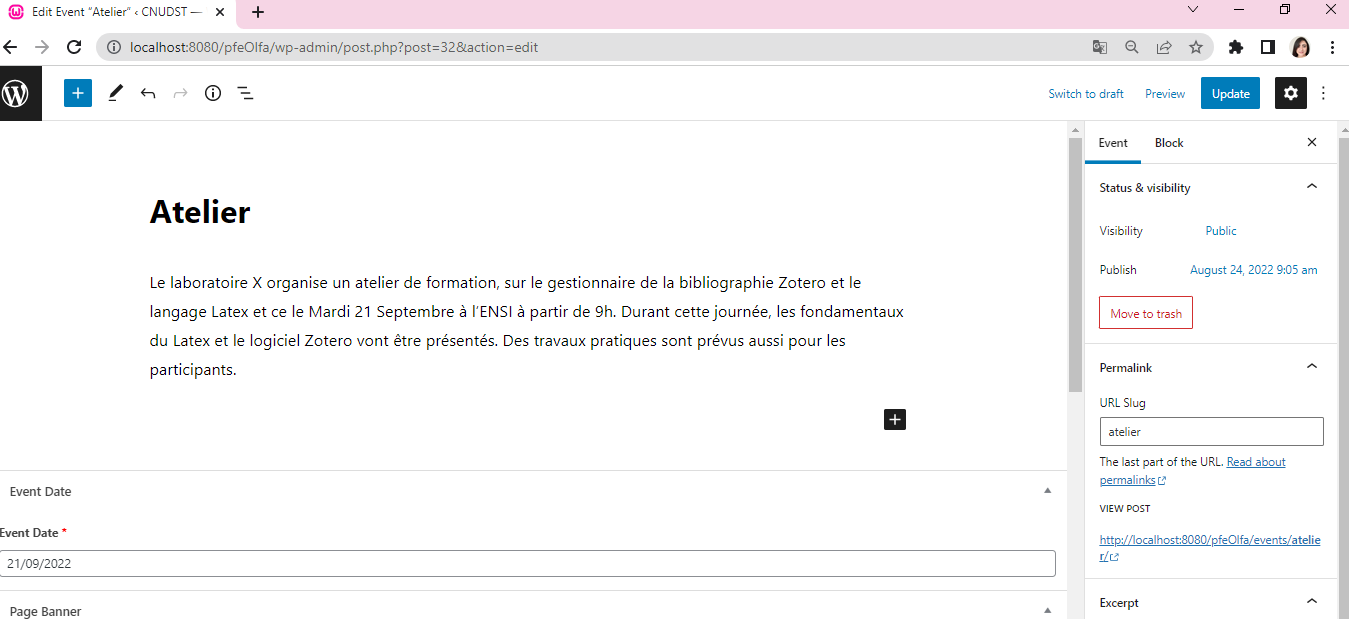
\includegraphics[width=1\textwidth]{D) IMAGES/Champs.png}}
	\caption{Ajouter les informations d'un thème}
	\label{Diagramme3}
\end{figure}
\newpage
Cette interface représentée par le schéma ci-dessus, permet à l'administrateur d'ajouter le titre d'un thème ainsi que sa description et de fixer sa date.

\begin{figure}[!h]
	\centering
	{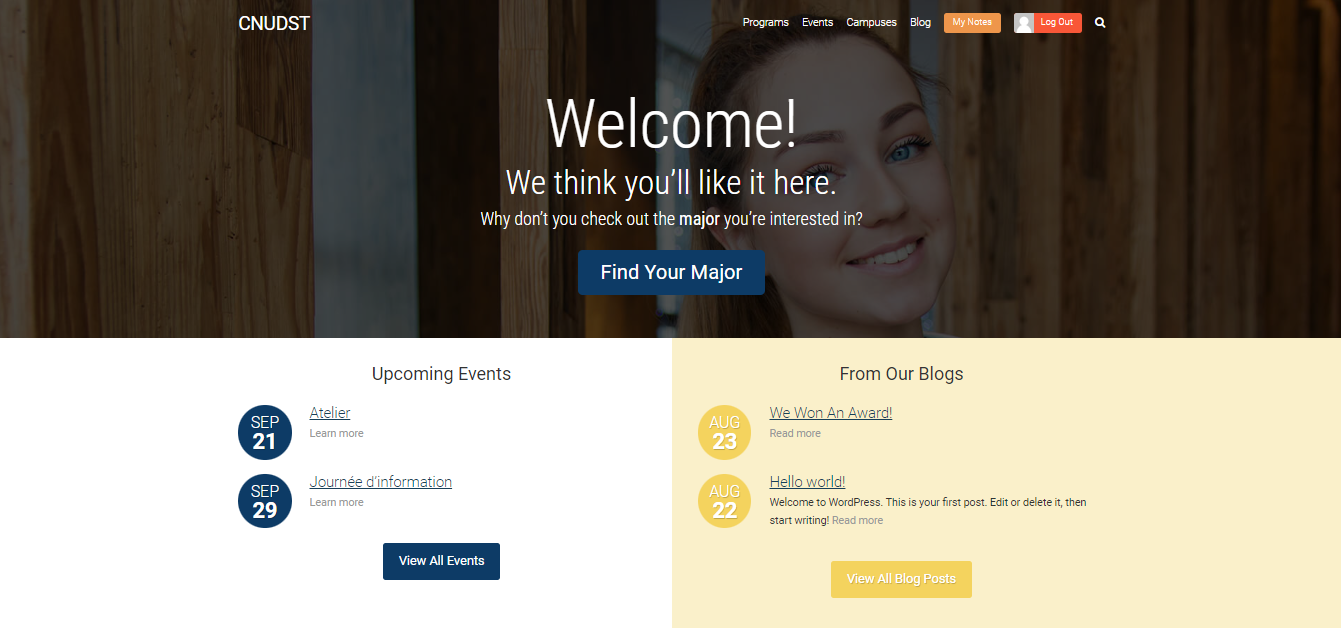
\includegraphics[width=1\textwidth]{D) IMAGES/ListerChamp.png}}
	\caption{Consulter thèmes}
	\label{Diagramme3}
\end{figure}
Cette page permet au visiteur de consulter la liste des thèmes en cliquant sur le bouton "View all Events" ou bien en utilisant l'onglet Events qui figure au niveau du menu.\\
\begin{figure}[!h]
	\centering
	{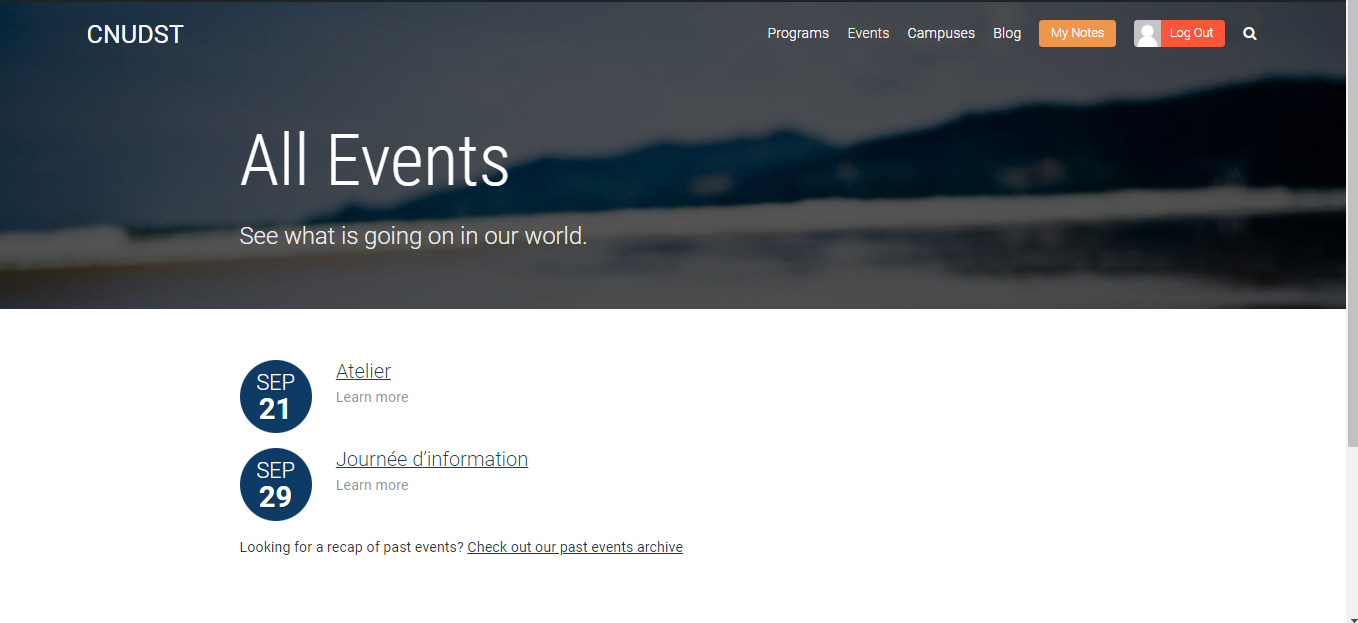
\includegraphics[width=1\textwidth]{D) IMAGES/BDlISTER.png}}
	\caption{Lister thèmes}
	\label{Diagramme3}
\end{figure}
\newpage
Cette interface permet au visiteur de lister l'ensemble des thèmes. Au niveau de cette page figure un lien qui permet au visiteur de consulter les thèmes passés.
\begin{figure}[!h]
	\centering
	{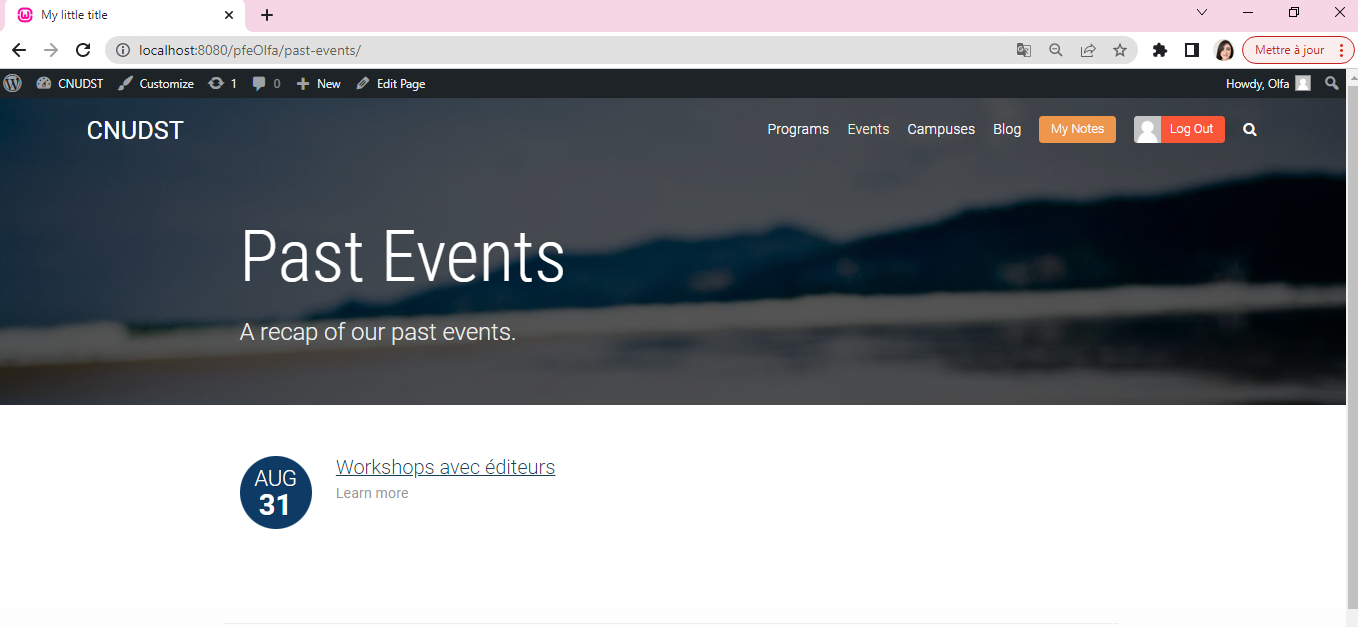
\includegraphics[width=1\textwidth]{D) IMAGES/Supprimer.png}}
	\caption{thèmes passés}
	\label{Diagramme3}
\end{figure}
\newpage
\begin{figure}[!h]
	\centering
	{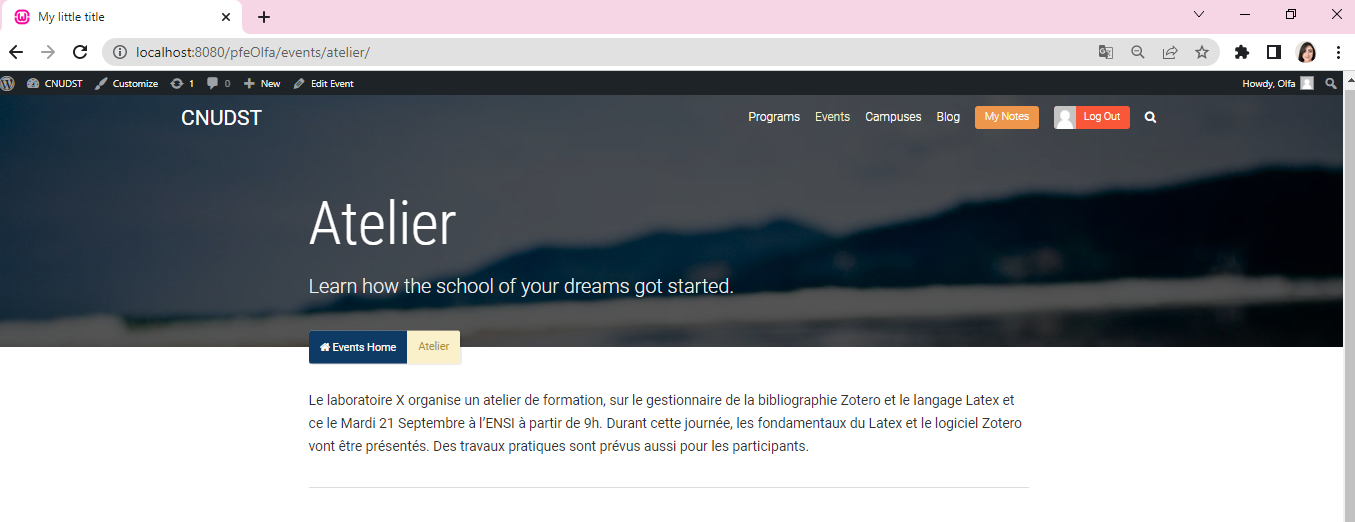
\includegraphics[width=1\textwidth]{D) IMAGES/Modifier.png}}
	\caption{Détails thème}
	\label{Diagramme3}
\end{figure}
Cette page permet d'afficher les détails d'un thème de formations.



\textbf{Conclusion}\\
A la fin de ce premier sprint qui a duré quatre semaines, nous avons pu livrer notre premier incrément. Pour y arriver nous avons effectué les étapes suivantes: le sprint planning meeting, l'analyse et la conception et la réalisation du produit.\\
Dans le chapitre suivant, nous allons entamer le deuxième sprint.




